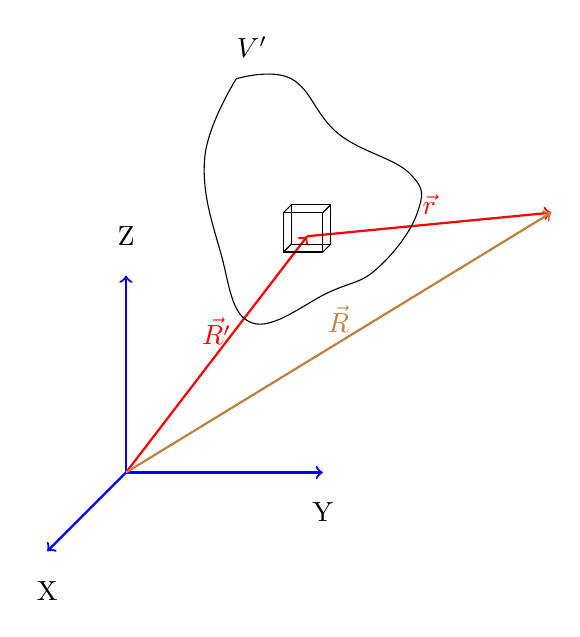
\begin{tikzpicture}
\draw [<->, blue, thick](-6.5,-4) -- (-6.5,-6.5) node (v1) {} -- (-4,-6.5);
\draw [->, blue, thick] (v1.center) -- (-7.5,-7.5);
\node at (-4,-7) {Y};
\node at (-7.5,-8) {X};
\node at (-6.5,-3.5) {Z};
\draw  [fill](-4.2,-3.5) node (v2) {} circle (0);
\draw [->, red, thick] (v1.center) -- (v2.center) node [midway, above]{$\vec{R'}$};
\draw [->, red, thick] (v2.center) -- (-1.1,-3.2) node [midway, above]{$\vec{r}$};
\draw [->, brown, thick] (v1.center) -- (-1.1,-3.2) node [midway, above]{$\vec{R}$};
\draw  (-4.5,-3.2) node (v4) {} rectangle (-4,-3.7) node (v6) {};
\draw  (-4.4,-3.1) node (v3) {} rectangle (-3.9,-3.6) node (v5) {};
\draw  plot[smooth, tension=.7] coordinates {(-5.1,-1.5) (-5.5,-2.5) (-5.3,-3.7) (-4.9,-4.6) (-3.9,-4.2) (-3.3,-3.9) (-2.8,-3.2) (-2.9,-2.7) (-3.8,-2.2) (-4.4,-1.5) (-5.1,-1.5)};
\node at (-4.9,-1.1) {$V'$};
\draw (-3.9,-3.1) -- (-4,-3.2);
\draw (-4.4,-3.6) -- (-4.5,-3.7);
\draw (v3.center) -- (v4.center);
\draw (v5.center) -- (v6.center);
\end{tikzpicture}